\documentclass[twoside]{book}

% Packages required by doxygen
\usepackage{fixltx2e}
\usepackage{calc}
\usepackage{doxygen}
\usepackage[export]{adjustbox} % also loads graphicx
\usepackage{graphicx}
\usepackage[utf8]{inputenc}
\usepackage{makeidx}
\usepackage{multicol}
\usepackage{multirow}
\PassOptionsToPackage{warn}{textcomp}
\usepackage{textcomp}
\usepackage[nointegrals]{wasysym}
\usepackage[table]{xcolor}

% Font selection
\usepackage[T1]{fontenc}
\usepackage[scaled=.90]{helvet}
\usepackage{courier}
\usepackage{amssymb}
\usepackage{sectsty}
\renewcommand{\familydefault}{\sfdefault}
\allsectionsfont{%
  \fontseries{bc}\selectfont%
  \color{darkgray}%
}
\renewcommand{\DoxyLabelFont}{%
  \fontseries{bc}\selectfont%
  \color{darkgray}%
}
\newcommand{\+}{\discretionary{\mbox{\scriptsize$\hookleftarrow$}}{}{}}

% Page & text layout
\usepackage{geometry}
\geometry{%
  a4paper,%
  top=2.5cm,%
  bottom=2.5cm,%
  left=2.5cm,%
  right=2.5cm%
}
\tolerance=750
\hfuzz=15pt
\hbadness=750
\setlength{\emergencystretch}{15pt}
\setlength{\parindent}{0cm}
\setlength{\parskip}{3ex plus 2ex minus 2ex}
\makeatletter
\renewcommand{\paragraph}{%
  \@startsection{paragraph}{4}{0ex}{-1.0ex}{1.0ex}{%
    \normalfont\normalsize\bfseries\SS@parafont%
  }%
}
\renewcommand{\subparagraph}{%
  \@startsection{subparagraph}{5}{0ex}{-1.0ex}{1.0ex}{%
    \normalfont\normalsize\bfseries\SS@subparafont%
  }%
}
\makeatother

% Headers & footers
\usepackage{fancyhdr}
\pagestyle{fancyplain}
\fancyhead[LE]{\fancyplain{}{\bfseries\thepage}}
\fancyhead[CE]{\fancyplain{}{}}
\fancyhead[RE]{\fancyplain{}{\bfseries\leftmark}}
\fancyhead[LO]{\fancyplain{}{\bfseries\rightmark}}
\fancyhead[CO]{\fancyplain{}{}}
\fancyhead[RO]{\fancyplain{}{\bfseries\thepage}}
\fancyfoot[LE]{\fancyplain{}{}}
\fancyfoot[CE]{\fancyplain{}{}}
\fancyfoot[RE]{\fancyplain{}{\bfseries\scriptsize Generated by Doxygen }}
\fancyfoot[LO]{\fancyplain{}{\bfseries\scriptsize Generated by Doxygen }}
\fancyfoot[CO]{\fancyplain{}{}}
\fancyfoot[RO]{\fancyplain{}{}}
\renewcommand{\footrulewidth}{0.4pt}
\renewcommand{\chaptermark}[1]{%
  \markboth{#1}{}%
}
\renewcommand{\sectionmark}[1]{%
  \markright{\thesection\ #1}%
}

% Indices & bibliography
\usepackage{natbib}
\usepackage[titles]{tocloft}
\setcounter{tocdepth}{3}
\setcounter{secnumdepth}{5}
\makeindex

% Hyperlinks (required, but should be loaded last)
\usepackage{ifpdf}
\ifpdf
  \usepackage[pdftex,pagebackref=true]{hyperref}
\else
  \usepackage[ps2pdf,pagebackref=true]{hyperref}
\fi
\hypersetup{%
  colorlinks=true,%
  linkcolor=blue,%
  citecolor=blue,%
  unicode%
}

% Custom commands
\newcommand{\clearemptydoublepage}{%
  \newpage{\pagestyle{empty}\cleardoublepage}%
}

\usepackage{caption}
\captionsetup{labelsep=space,justification=centering,font={bf},singlelinecheck=off,skip=4pt,position=top}

%===== C O N T E N T S =====

\begin{document}

% Titlepage & ToC
\hypersetup{pageanchor=false,
             bookmarksnumbered=true,
             pdfencoding=unicode
            }
\pagenumbering{roman}
\begin{titlepage}
\vspace*{7cm}
\begin{center}%
{\Large P\+PP Assignment }\\
\vspace*{1cm}
{\large Generated by Doxygen 1.8.11}\\
\end{center}
\end{titlepage}
\clearemptydoublepage
\tableofcontents
\clearemptydoublepage
\pagenumbering{arabic}
\hypersetup{pageanchor=true}

%--- Begin generated contents ---
\chapter{Hierarchical Index}
\section{Class Hierarchy}
This inheritance list is sorted roughly, but not completely, alphabetically\+:\begin{DoxyCompactList}
\item \contentsline{section}{Game\+Object}{\pageref{classGameObject}}{}
\begin{DoxyCompactList}
\item \contentsline{section}{Bullet}{\pageref{classBullet}}{}
\item \contentsline{section}{Enemy}{\pageref{classEnemy}}{}
\begin{DoxyCompactList}
\item \contentsline{section}{Enemy\+Satellite}{\pageref{classEnemySatellite}}{}
\end{DoxyCompactList}
\item \contentsline{section}{Obstacle}{\pageref{classObstacle}}{}
\item \contentsline{section}{Player}{\pageref{classPlayer}}{}
\end{DoxyCompactList}
\item \contentsline{section}{G\+L\+Functions}{\pageref{classGLFunctions}}{}
\item \contentsline{section}{Level}{\pageref{classLevel}}{}
\item \contentsline{section}{Mat4}{\pageref{classMat4}}{}
\item \contentsline{section}{Mesh}{\pageref{classMesh}}{}
\item \contentsline{section}{Particle}{\pageref{classParticle}}{}
\item \contentsline{section}{Particles}{\pageref{classParticles}}{}
\item \contentsline{section}{Utility\+Functions}{\pageref{classUtilityFunctions}}{}
\item \contentsline{section}{utility\+Functions}{\pageref{classutilityFunctions}}{}
\item \contentsline{section}{Vec4}{\pageref{classVec4}}{}
\item \contentsline{section}{Window}{\pageref{classWindow}}{}
\end{DoxyCompactList}

\chapter{Class Index}
\section{Class List}
Here are the classes, structs, unions and interfaces with brief descriptions\+:\begin{DoxyCompactList}
\item\contentsline{section}{\hyperlink{classBullet}{Bullet} \\*Bullets that can be shot by players or enemies }{\pageref{classBullet}}{}
\item\contentsline{section}{\hyperlink{classEnemy}{Enemy} \\*Gameobjects hostile to the player }{\pageref{classEnemy}}{}
\item\contentsline{section}{\hyperlink{classEnemySatellite}{Enemy\+Satellite} \\*Enemies that rotate around a defined point }{\pageref{classEnemySatellite}}{}
\item\contentsline{section}{\hyperlink{classGameObject}{Game\+Object} \\*This class is the base class for most of the objects in the scene }{\pageref{classGameObject}}{}
\item\contentsline{section}{\hyperlink{classGLFunctions}{G\+L\+Functions} }{\pageref{classGLFunctions}}{}
\item\contentsline{section}{\hyperlink{classLevel}{Level} \\*Most objects, it is basically a \char`\"{}master class\char`\"{}, which was useful to manage timers }{\pageref{classLevel}}{}
\item\contentsline{section}{\hyperlink{classMat4}{Mat4} }{\pageref{classMat4}}{}
\item\contentsline{section}{\hyperlink{classMesh}{Mesh} \\*Data imported from a .O\+BJ file }{\pageref{classMesh}}{}
\item\contentsline{section}{\hyperlink{classObstacle}{Obstacle} \\*Inherits from \hyperlink{classGameObject}{Game\+Object} and is a static element in the scene }{\pageref{classObstacle}}{}
\item\contentsline{section}{\hyperlink{classParticle}{Particle} \\*Single element that will move in the same direction at constant speed }{\pageref{classParticle}}{}
\item\contentsline{section}{\hyperlink{classParticles}{Particles} \\*Handles the activation of multiple \hyperlink{classParticle}{Particle} objects }{\pageref{classParticles}}{}
\item\contentsline{section}{\hyperlink{classPlayer}{Player} \\*Object controlled by a player }{\pageref{classPlayer}}{}
\item\contentsline{section}{\hyperlink{classUtilityFunctions}{Utility\+Functions} \\*Bundle of functions that helped me in the developement process }{\pageref{classUtilityFunctions}}{}
\item\contentsline{section}{\hyperlink{classutilityFunctions}{utility\+Functions} }{\pageref{classutilityFunctions}}{}
\item\contentsline{section}{\hyperlink{classVec4}{Vec4} }{\pageref{classVec4}}{}
\item\contentsline{section}{\hyperlink{classWindow}{Window} \\*Initializes Open\+GL and S\+DL and creates a window }{\pageref{classWindow}}{}
\end{DoxyCompactList}

\chapter{Class Documentation}
\hypertarget{classBullet}{}\section{Bullet Class Reference}
\label{classBullet}\index{Bullet@{Bullet}}


bullets that can be shot by players or enemies  




{\ttfamily \#include $<$Bullet.\+h$>$}

Inheritance diagram for Bullet\+:\begin{figure}[H]
\begin{center}
\leavevmode
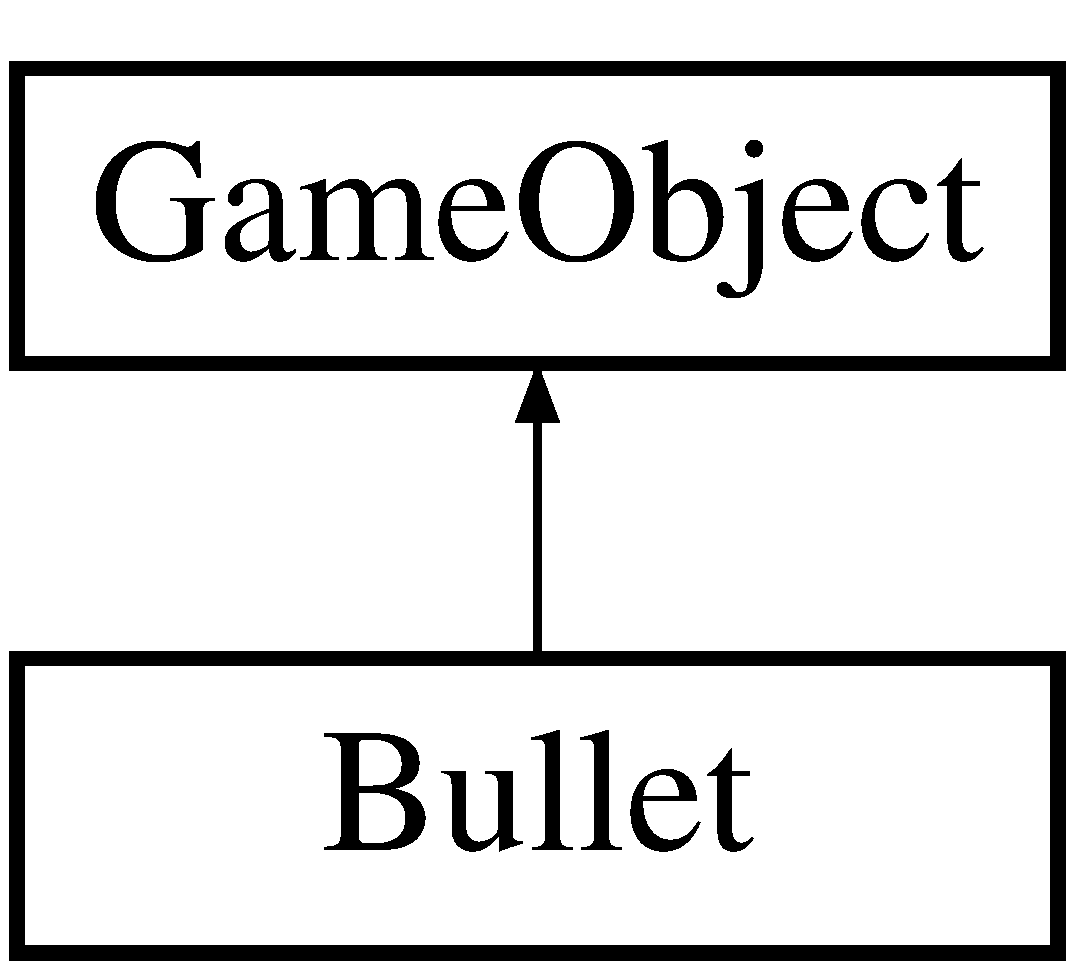
\includegraphics[height=2.000000cm]{classBullet}
\end{center}
\end{figure}
\subsection*{Public Member Functions}
\begin{DoxyCompactItemize}
\item 
{\bfseries Bullet} (const \hyperlink{classVec4}{Vec4} \+\_\+position, const \hyperlink{classVec4}{Vec4} \+\_\+rotation, float \+\_\+speed, bool \+\_\+active, \hyperlink{classMesh}{Mesh} $\ast$\+\_\+mesh)\hypertarget{classBullet_a69a901bd61482d283deb9ba0815fe088}{}\label{classBullet_a69a901bd61482d283deb9ba0815fe088}

\item 
void {\bfseries set\+Parent} (\hyperlink{classGameObject}{Game\+Object} $\ast$\+\_\+parent)\hypertarget{classBullet_ab987516db817716708d347ff07a1ec00}{}\label{classBullet_ab987516db817716708d347ff07a1ec00}

\item 
void {\bfseries active} (bool const \+\_\+active)\hypertarget{classBullet_a7db83333ebb09d7ab2ac402b65df86b1}{}\label{classBullet_a7db83333ebb09d7ab2ac402b65df86b1}

\item 
bool {\bfseries active} () const \hypertarget{classBullet_ab984176acb53a108101208b02274efde}{}\label{classBullet_ab984176acb53a108101208b02274efde}

\item 
void {\bfseries update\+Position} () override\hypertarget{classBullet_aaf18157aae6a1e6d2296090bb705dd18}{}\label{classBullet_aaf18157aae6a1e6d2296090bb705dd18}

\item 
void {\bfseries draw} () const \hypertarget{classBullet_ac11bd30a1ad0a983504aed51525bed13}{}\label{classBullet_ac11bd30a1ad0a983504aed51525bed13}

\item 
\hyperlink{classGameObject}{Game\+Object} $\ast$ {\bfseries get\+Parent} ()\hypertarget{classBullet_a3393efe36b297d896b863993b28985d2}{}\label{classBullet_a3393efe36b297d896b863993b28985d2}

\end{DoxyCompactItemize}
\subsection*{Additional Inherited Members}


\subsection{Detailed Description}
bullets that can be shot by players or enemies 

The documentation for this class was generated from the following file\+:\begin{DoxyCompactItemize}
\item 
include/Bullet.\+h\end{DoxyCompactItemize}

\hypertarget{classEnemy}{}\section{Enemy Class Reference}
\label{classEnemy}\index{Enemy@{Enemy}}


gameobjects hostile to the player  




{\ttfamily \#include $<$Enemy.\+h$>$}

Inheritance diagram for Enemy\+:\begin{figure}[H]
\begin{center}
\leavevmode
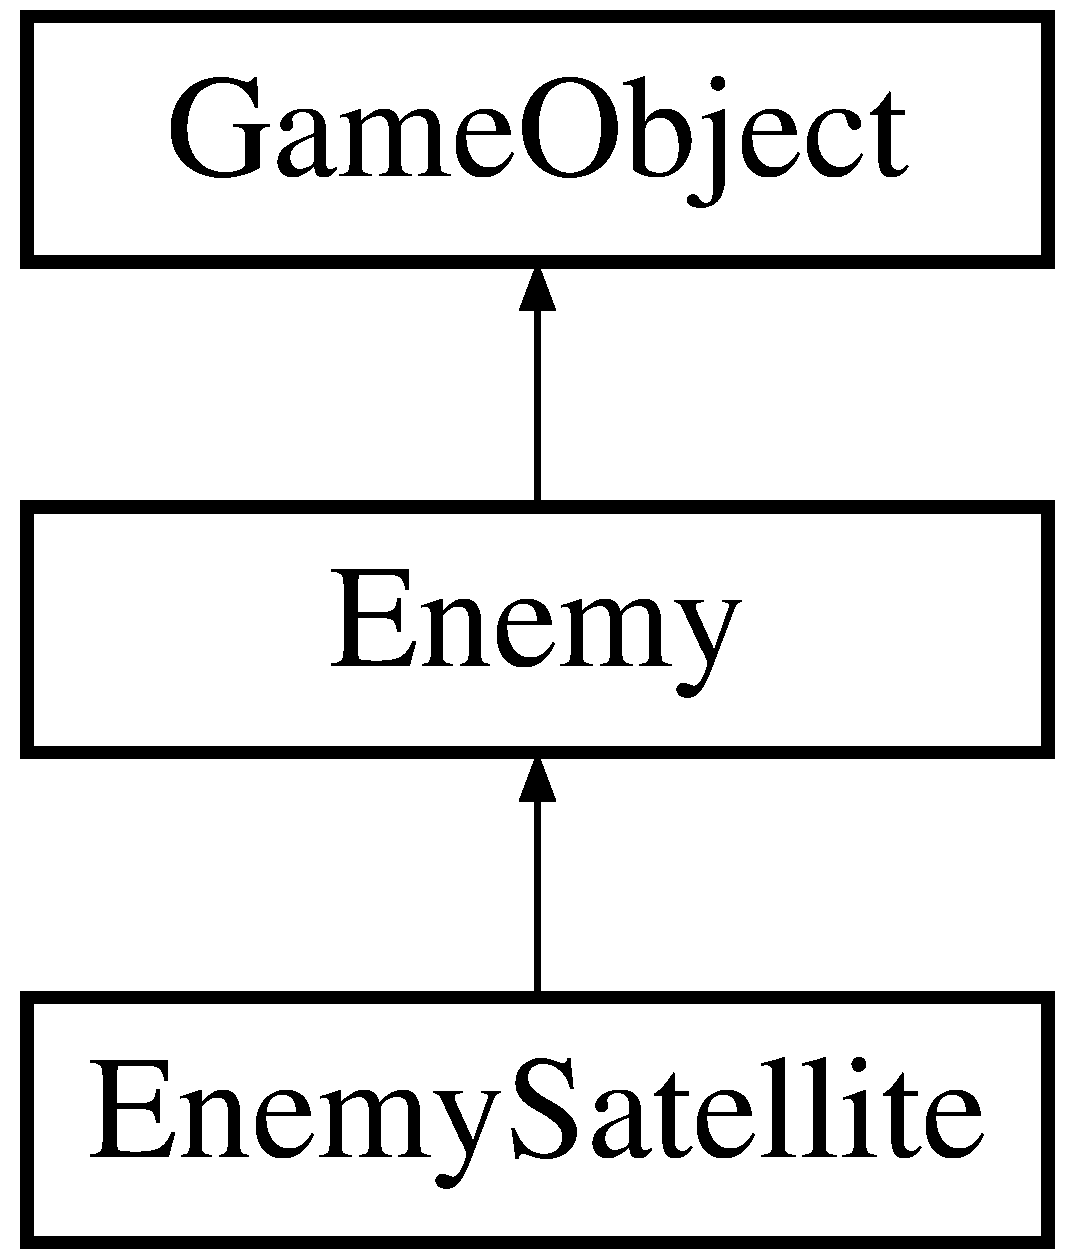
\includegraphics[height=3.000000cm]{classEnemy}
\end{center}
\end{figure}
\subsection*{Public Member Functions}
\begin{DoxyCompactItemize}
\item 
{\bfseries Enemy} (\hyperlink{classVec4}{Vec4} const \+\_\+position, \hyperlink{classVec4}{Vec4} const \+\_\+rotation, float \+\_\+speed, bool \+\_\+active, int \+\_\+life, \hyperlink{classMesh}{Mesh} $\ast$\+\_\+mesh, \hyperlink{classPlayer}{Player} $\ast$\+\_\+player)\hypertarget{classEnemy_ab74657627d71aa9644791fa8a2996f10}{}\label{classEnemy_ab74657627d71aa9644791fa8a2996f10}

\item 
virtual void {\bfseries update\+Position} ()\hypertarget{classEnemy_abca865a60e8134aa3fcfc4558de71587}{}\label{classEnemy_abca865a60e8134aa3fcfc4558de71587}

\item 
virtual void {\bfseries update\+Rotation} ()\hypertarget{classEnemy_a469a2e96ff4c742b7f4a13f1e12602a7}{}\label{classEnemy_a469a2e96ff4c742b7f4a13f1e12602a7}

\item 
virtual void {\bfseries draw} () const \hypertarget{classEnemy_a80f897d499f4caa87a161de4ba0ecde0}{}\label{classEnemy_a80f897d499f4caa87a161de4ba0ecde0}

\item 
bool {\bfseries can\+Shoot} () const \hypertarget{classEnemy_aec557d07779498d06946e448b4365bae}{}\label{classEnemy_aec557d07779498d06946e448b4365bae}

\item 
void {\bfseries can\+Shoot} (bool \+\_\+can\+Shoot)\hypertarget{classEnemy_a31998103d6c9d3aa5ed98ca9e2c11afb}{}\label{classEnemy_a31998103d6c9d3aa5ed98ca9e2c11afb}

\end{DoxyCompactItemize}
\subsection*{Protected Attributes}
\begin{DoxyCompactItemize}
\item 
bool {\bfseries m\+\_\+shoot}\hypertarget{classEnemy_a0adddde568ab04784f55483345a8a91f}{}\label{classEnemy_a0adddde568ab04784f55483345a8a91f}

\item 
\hyperlink{classMesh}{Mesh} $\ast$ {\bfseries m\+\_\+mesh}\hypertarget{classEnemy_afebfefd6f39ac7e7ff50a973861de65b}{}\label{classEnemy_afebfefd6f39ac7e7ff50a973861de65b}

\item 
\hyperlink{classPlayer}{Player} $\ast$ {\bfseries m\+\_\+player}\hypertarget{classEnemy_a98d4492b5b0884704a8bf30d3f53108c}{}\label{classEnemy_a98d4492b5b0884704a8bf30d3f53108c}

\item 
float {\bfseries m\+\_\+size}\hypertarget{classEnemy_abc4b39ceb10b8f9741b41c22cd0c6554}{}\label{classEnemy_abc4b39ceb10b8f9741b41c22cd0c6554}

\item 
bool {\bfseries m\+\_\+can\+Shoot}\hypertarget{classEnemy_a387cb17e4c46c8e8663b6313e0962274}{}\label{classEnemy_a387cb17e4c46c8e8663b6313e0962274}

\item 
bool {\bfseries m\+\_\+close\+To\+Player}\hypertarget{classEnemy_a3801f0224fad82ac775a371b4c576e0c}{}\label{classEnemy_a3801f0224fad82ac775a371b4c576e0c}

\end{DoxyCompactItemize}


\subsection{Detailed Description}
gameobjects hostile to the player 

The documentation for this class was generated from the following file\+:\begin{DoxyCompactItemize}
\item 
include/Enemy.\+h\end{DoxyCompactItemize}

\hypertarget{classEnemySatellite}{}\section{Enemy\+Satellite Class Reference}
\label{classEnemySatellite}\index{Enemy\+Satellite@{Enemy\+Satellite}}


Enemies that rotate around a defined point.  




{\ttfamily \#include $<$Enemy\+Satellite.\+h$>$}

Inheritance diagram for Enemy\+Satellite\+:\begin{figure}[H]
\begin{center}
\leavevmode
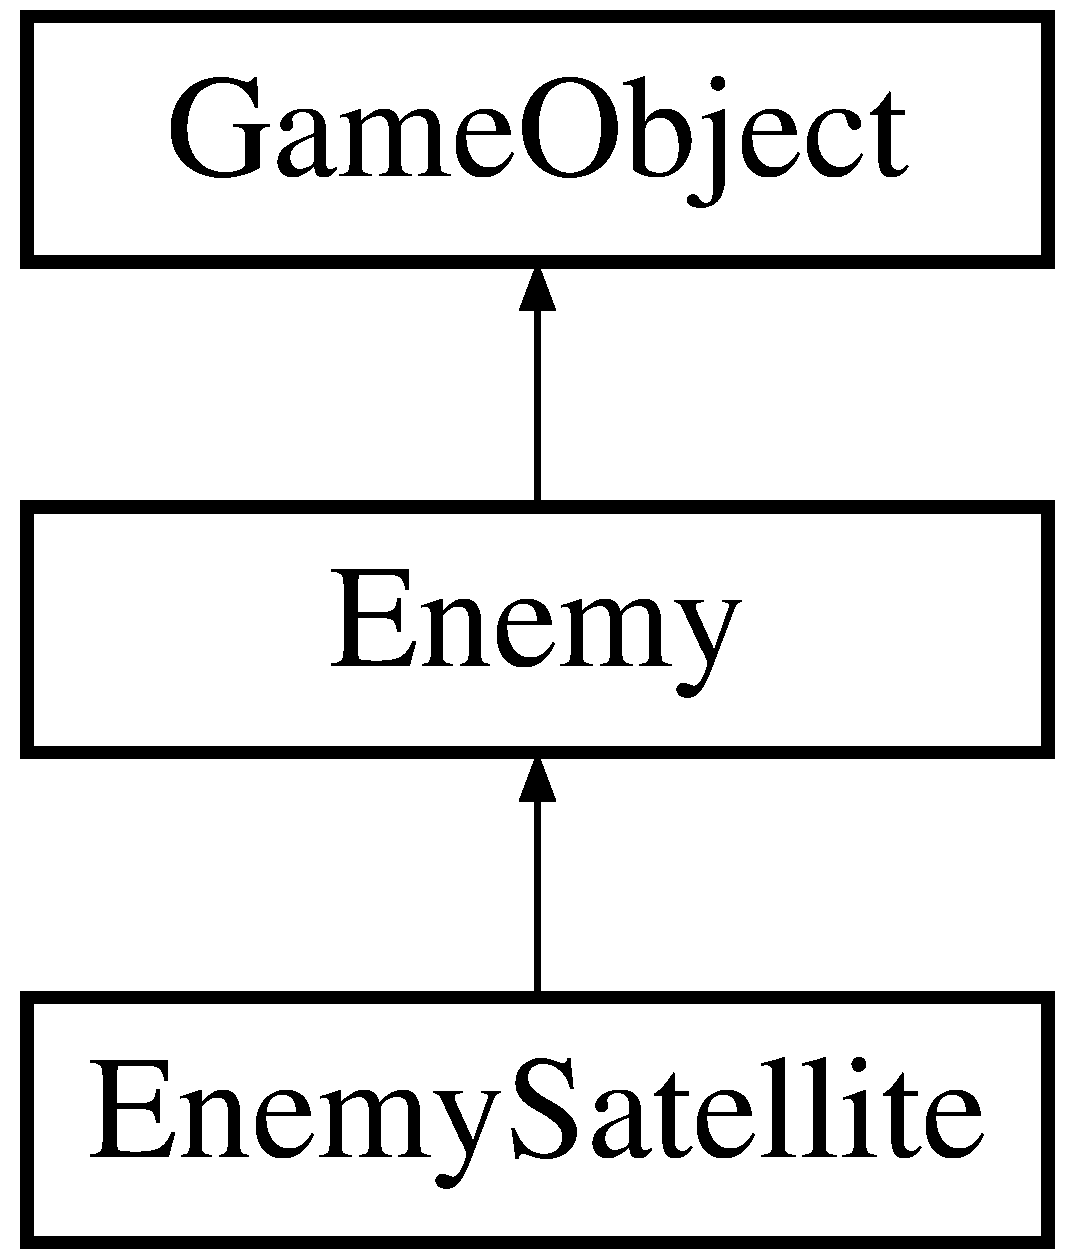
\includegraphics[height=3.000000cm]{classEnemySatellite}
\end{center}
\end{figure}
\subsection*{Public Member Functions}
\begin{DoxyCompactItemize}
\item 
{\bfseries Enemy\+Satellite} (\hyperlink{classVec4}{Vec4} \+\_\+position, \hyperlink{classVec4}{Vec4} \+\_\+center, \hyperlink{classMesh}{Mesh} $\ast$\+\_\+mesh, \hyperlink{classPlayer}{Player} $\ast$\+\_\+player, float \+\_\+speed, bool \+\_\+active, int \+\_\+life)\hypertarget{classEnemySatellite_af58da30acb9af47b7d40ae80b76008e8}{}\label{classEnemySatellite_af58da30acb9af47b7d40ae80b76008e8}

\item 
void {\bfseries update\+Position} () override\hypertarget{classEnemySatellite_a07c15081994ca6f402659ffd5ac771b4}{}\label{classEnemySatellite_a07c15081994ca6f402659ffd5ac771b4}

\end{DoxyCompactItemize}
\subsection*{Additional Inherited Members}


\subsection{Detailed Description}
Enemies that rotate around a defined point. 

The documentation for this class was generated from the following file\+:\begin{DoxyCompactItemize}
\item 
include/Enemy\+Satellite.\+h\end{DoxyCompactItemize}

\hypertarget{classGameObject}{}\section{Game\+Object Class Reference}
\label{classGameObject}\index{Game\+Object@{Game\+Object}}


this class is the base class for most of the objects in the scene  




{\ttfamily \#include $<$Game\+Object.\+h$>$}

Inheritance diagram for Game\+Object\+:\begin{figure}[H]
\begin{center}
\leavevmode
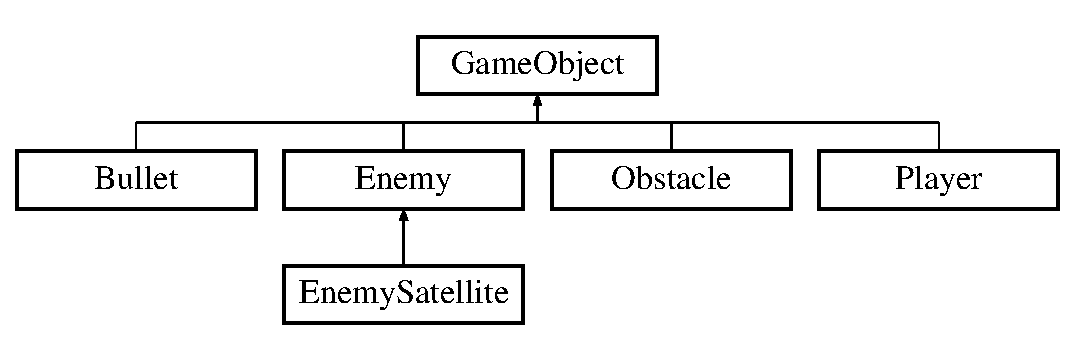
\includegraphics[height=3.000000cm]{classGameObject}
\end{center}
\end{figure}
\subsection*{Public Member Functions}
\begin{DoxyCompactItemize}
\item 
{\bfseries Game\+Object} (const \hyperlink{classVec4}{Vec4} \+\_\+position, const \hyperlink{classVec4}{Vec4} \+\_\+rotation, float \+\_\+speed, bool \+\_\+active)\hypertarget{classGameObject_a89fec6ab796fa6a89a7b7f575b3636b2}{}\label{classGameObject_a89fec6ab796fa6a89a7b7f575b3636b2}

\item 
virtual void {\bfseries update\+Position} ()\hypertarget{classGameObject_a889e4c64a347b028dfc08f2d07d74941}{}\label{classGameObject_a889e4c64a347b028dfc08f2d07d74941}

\item 
virtual void {\bfseries update\+Rotation} ()\hypertarget{classGameObject_a3d7da3a084131542410978e7fe4014be}{}\label{classGameObject_a3d7da3a084131542410978e7fe4014be}

\item 
virtual bool {\bfseries active} () const \hypertarget{classGameObject_a70fc35dbbeb50ccf6e8ff7d3bc7d1d02}{}\label{classGameObject_a70fc35dbbeb50ccf6e8ff7d3bc7d1d02}

\item 
virtual void {\bfseries active} (bool const \+\_\+active)\hypertarget{classGameObject_a0411665392a0af17c2da5364da9a4e2e}{}\label{classGameObject_a0411665392a0af17c2da5364da9a4e2e}

\item 
virtual void {\bfseries check\+Collision} (bool \+\_\+collided)\hypertarget{classGameObject_aed8abb63dd5ac35f712fa3635d37a6b1}{}\label{classGameObject_aed8abb63dd5ac35f712fa3635d37a6b1}

\item 
virtual void {\bfseries draw} () const \hypertarget{classGameObject_a288d4de0d98d836880f73d70dc98e14b}{}\label{classGameObject_a288d4de0d98d836880f73d70dc98e14b}

\item 
int {\bfseries life} () const \hypertarget{classGameObject_a50dbeccde2372724014b19bcf47d1d57}{}\label{classGameObject_a50dbeccde2372724014b19bcf47d1d57}

\item 
void {\bfseries life} (int const \+\_\+life)\hypertarget{classGameObject_a1a01cd7deaecc0f5db3d8aaf6c33cde8}{}\label{classGameObject_a1a01cd7deaecc0f5db3d8aaf6c33cde8}

\item 
\hyperlink{classVec4}{Vec4} {\bfseries get\+Position} () const \hypertarget{classGameObject_a7b738ea488607268c09123402dd6099a}{}\label{classGameObject_a7b738ea488607268c09123402dd6099a}

\item 
\hyperlink{classVec4}{Vec4} {\bfseries get\+Rotation} () const \hypertarget{classGameObject_a8123d06d5ef29528b0bf1c3999b342fd}{}\label{classGameObject_a8123d06d5ef29528b0bf1c3999b342fd}

\item 
float {\bfseries get\+Collision\+Limit\+\_\+x} () const \hypertarget{classGameObject_ae2c30d83ab2851b0103a2341a8d45a67}{}\label{classGameObject_ae2c30d83ab2851b0103a2341a8d45a67}

\item 
float {\bfseries get\+Collision\+Limit\+\_\+z} () const \hypertarget{classGameObject_aa09cdfc6bd31ea886167c2fa800a418f}{}\label{classGameObject_aa09cdfc6bd31ea886167c2fa800a418f}

\item 
float {\bfseries get\+Size} () const \hypertarget{classGameObject_af8ce553742a98ea7a4dd124aca953465}{}\label{classGameObject_af8ce553742a98ea7a4dd124aca953465}

\end{DoxyCompactItemize}
\subsection*{Protected Attributes}
\begin{DoxyCompactItemize}
\item 
\hyperlink{classVec4}{Vec4} {\bfseries m\+\_\+position}\hypertarget{classGameObject_a3173b6cca3aa6b1d3d6989fd4bfb7b40}{}\label{classGameObject_a3173b6cca3aa6b1d3d6989fd4bfb7b40}

\item 
\hyperlink{classVec4}{Vec4} {\bfseries m\+\_\+rotation}\hypertarget{classGameObject_a1af7cd3ccd584b494b84cb8d1128abaf}{}\label{classGameObject_a1af7cd3ccd584b494b84cb8d1128abaf}

\item 
float {\bfseries m\+\_\+speed}\hypertarget{classGameObject_a1e3d1c84dbf06473b5f058ec032b859a}{}\label{classGameObject_a1e3d1c84dbf06473b5f058ec032b859a}

\item 
float {\bfseries m\+\_\+size}\hypertarget{classGameObject_a707df0ee16fc77ceed35015b1d739de2}{}\label{classGameObject_a707df0ee16fc77ceed35015b1d739de2}

\item 
float {\bfseries m\+\_\+life}\hypertarget{classGameObject_acc140236510083ff31d931dba9f90ba3}{}\label{classGameObject_acc140236510083ff31d931dba9f90ba3}

\item 
float {\bfseries m\+\_\+collision\+Limit\+\_\+x}\hypertarget{classGameObject_a988655066d614a89f3614f823fb38d2b}{}\label{classGameObject_a988655066d614a89f3614f823fb38d2b}

\item 
float {\bfseries m\+\_\+collision\+Limit\+\_\+z}\hypertarget{classGameObject_a801cd4461df690e0ef4a4311ca7ec26d}{}\label{classGameObject_a801cd4461df690e0ef4a4311ca7ec26d}

\item 
bool {\bfseries m\+\_\+active}\hypertarget{classGameObject_a65307073834455243a8b339592245603}{}\label{classGameObject_a65307073834455243a8b339592245603}

\item 
bool {\bfseries m\+\_\+collided}\hypertarget{classGameObject_a5fac043e6844df16e5ccaf5ffaaab5bd}{}\label{classGameObject_a5fac043e6844df16e5ccaf5ffaaab5bd}

\end{DoxyCompactItemize}


\subsection{Detailed Description}
this class is the base class for most of the objects in the scene 

The documentation for this class was generated from the following file\+:\begin{DoxyCompactItemize}
\item 
include/Game\+Object.\+h\end{DoxyCompactItemize}

\hypertarget{classGLFunctions}{}\section{G\+L\+Functions Class Reference}
\label{classGLFunctions}\index{G\+L\+Functions@{G\+L\+Functions}}
\subsection*{Static Public Member Functions}
\begin{DoxyCompactItemize}
\item 
static void {\bfseries cube} (G\+Lfloat \+\_\+w, G\+Lfloat \+\_\+h, G\+Lfloat \+\_\+d)\hypertarget{classGLFunctions_aee5b3f390ec85d0d414292d0ed7255a3}{}\label{classGLFunctions_aee5b3f390ec85d0d414292d0ed7255a3}

\item 
static void {\bfseries look\+At} (\hyperlink{classVec4}{Vec4} \+\_\+eye, \hyperlink{classVec4}{Vec4} \+\_\+look, \hyperlink{classVec4}{Vec4} \+\_\+up)\hypertarget{classGLFunctions_a1c20e262bc92cfecb3d9465b8f87f0f6}{}\label{classGLFunctions_a1c20e262bc92cfecb3d9465b8f87f0f6}

\item 
static void {\bfseries perspective} (float \+\_\+fovy, float \+\_\+aspect, float \+\_\+z\+Near, float \+\_\+z\+Far)\hypertarget{classGLFunctions_abd3c398c9beea93c4f213e8f8ad53e06}{}\label{classGLFunctions_abd3c398c9beea93c4f213e8f8ad53e06}

\item 
static float {\bfseries radians} (float \+\_\+deg)\hypertarget{classGLFunctions_a5a15e7a581ababd7bdc810d15422612d}{}\label{classGLFunctions_a5a15e7a581ababd7bdc810d15422612d}

\item 
static void {\bfseries sphere} (float \+\_\+radius, int \+\_\+precision)\hypertarget{classGLFunctions_ab6916b1ff59f14bd1926c6b56069b460}{}\label{classGLFunctions_ab6916b1ff59f14bd1926c6b56069b460}

\item 
static void {\bfseries capsule} (float \+\_\+radius, float \+\_\+height, int \+\_\+precision)\hypertarget{classGLFunctions_a1dec6aa52e2bda58ab28bba2b574243c}{}\label{classGLFunctions_a1dec6aa52e2bda58ab28bba2b574243c}

\item 
static void {\bfseries cylinder} (float \+\_\+radius, const float \+\_\+height, int \+\_\+slices, int \+\_\+stacks)\hypertarget{classGLFunctions_ae4ccc483de859724e6fe8b8152b7b0af}{}\label{classGLFunctions_ae4ccc483de859724e6fe8b8152b7b0af}

\item 
static void {\bfseries cone} (float \+\_\+base, float \+\_\+height, int \+\_\+slices, int \+\_\+stacks)\hypertarget{classGLFunctions_a471fd78e978c74b54fd54f4b240341a2}{}\label{classGLFunctions_a471fd78e978c74b54fd54f4b240341a2}

\item 
static void {\bfseries disk} (float \+\_\+radius, int \+\_\+slices)\hypertarget{classGLFunctions_aca7c72689f74beb6e6bd5a296f96155f}{}\label{classGLFunctions_aca7c72689f74beb6e6bd5a296f96155f}

\item 
static void {\bfseries torus} (float \+\_\+minor\+Radius, float \+\_\+major\+Radius, int \+\_\+n\+Sides, int \+\_\+n\+Rings)\hypertarget{classGLFunctions_ae15d01f8935596011c0bdf3a9f604607}{}\label{classGLFunctions_ae15d01f8935596011c0bdf3a9f604607}

\end{DoxyCompactItemize}


The documentation for this class was generated from the following file\+:\begin{DoxyCompactItemize}
\item 
G\+L\+Functions\+Lib/include/G\+L\+Functions.\+h\end{DoxyCompactItemize}

\hypertarget{classLevel}{}\section{Level Class Reference}
\label{classLevel}\index{Level@{Level}}


contains most objects, it is basically a \char`\"{}master class\char`\"{}, which was useful to manage timers  




{\ttfamily \#include $<$Level.\+h$>$}

\subsection*{Public Member Functions}
\begin{DoxyCompactItemize}
\item 
{\bfseries Level} (std\+::string \+\_\+address, \hyperlink{classPlayer}{Player} $\ast$\+\_\+player, std\+::vector$<$ \hyperlink{classMesh}{Mesh} $\ast$ $>$ \+\_\+meshes, int \+\_\+cell\+Size)\hypertarget{classLevel_ad43f3f39d70bce7065f5bbd299b43d74}{}\label{classLevel_ad43f3f39d70bce7065f5bbd299b43d74}

\item 
void {\bfseries draw\+Map} () const \hypertarget{classLevel_a522a8acb3610c8e02b3063b098ea6c9a}{}\label{classLevel_a522a8acb3610c8e02b3063b098ea6c9a}

\item 
void {\bfseries draw} () const \hypertarget{classLevel_ae7de8e9ecd7d33a6b891bf58f3a71951}{}\label{classLevel_ae7de8e9ecd7d33a6b891bf58f3a71951}

\item 
bool {\bfseries wall\+Collision} (\hyperlink{classGameObject}{Game\+Object} $\ast$\+\_\+game\+Object, \hyperlink{classVec4}{Vec4} \+\_\+pos)\hypertarget{classLevel_a6b93a8960e619d24e0a76d877be1f36e}{}\label{classLevel_a6b93a8960e619d24e0a76d877be1f36e}

\item 
void {\bfseries update} ()\hypertarget{classLevel_a62e412eaad753d2baa2f94239cb80e41}{}\label{classLevel_a62e412eaad753d2baa2f94239cb80e41}

\item 
void {\bfseries activate\+Bullets} ()\hypertarget{classLevel_a3a0dd3f0d9936cbb44b2de0283b94200}{}\label{classLevel_a3a0dd3f0d9936cbb44b2de0283b94200}

\item 
void {\bfseries Collisions} ()\hypertarget{classLevel_ab9335b7276b912dce033d4b57e56f5c9}{}\label{classLevel_ab9335b7276b912dce033d4b57e56f5c9}

\item 
\hyperlink{classPlayer}{Player} $\ast$ {\bfseries get\+Player} ()\hypertarget{classLevel_a583930f5b9967473062f8f3abdc780ef}{}\label{classLevel_a583930f5b9967473062f8f3abdc780ef}

\item 
void {\bfseries enemy\+Can\+Shoot} ()\hypertarget{classLevel_a20349e0b0cd045abcbc879f2ed38e5e4}{}\label{classLevel_a20349e0b0cd045abcbc879f2ed38e5e4}

\item 
\hyperlink{classParticles}{Particles} $\ast$ {\bfseries get\+Particles} ()\hypertarget{classLevel_aef4b5e429a6ca396591dc2014d088b2c}{}\label{classLevel_aef4b5e429a6ca396591dc2014d088b2c}

\end{DoxyCompactItemize}


\subsection{Detailed Description}
contains most objects, it is basically a \char`\"{}master class\char`\"{}, which was useful to manage timers 

The documentation for this class was generated from the following file\+:\begin{DoxyCompactItemize}
\item 
include/Level.\+h\end{DoxyCompactItemize}

\hypertarget{classMat4}{}\section{Mat4 Class Reference}
\label{classMat4}\index{Mat4@{Mat4}}
\subsection*{Public Member Functions}
\begin{DoxyCompactItemize}
\item 
{\bfseries Mat4} (G\+Lfloat \+\_\+s=1.\+0f)\hypertarget{classMat4_ae851bfadb8c8bec37790dd3ffe03a126}{}\label{classMat4_ae851bfadb8c8bec37790dd3ffe03a126}

\item 
{\bfseries Mat4} (const \hyperlink{classMat4}{Mat4} \&r)=default\hypertarget{classMat4_ac1cd126926de151f53dfd568afce1152}{}\label{classMat4_ac1cd126926de151f53dfd568afce1152}

\item 
void {\bfseries operator$\ast$=} (const \hyperlink{classMat4}{Mat4} \&\+\_\+rhs)\hypertarget{classMat4_a5b8ca6003dee9d49f2a008f1608bebaf}{}\label{classMat4_a5b8ca6003dee9d49f2a008f1608bebaf}

\item 
\hyperlink{classMat4}{Mat4} {\bfseries operator$\ast$} (const \hyperlink{classMat4}{Mat4} \&\+\_\+rhs) const \hypertarget{classMat4_a354d63d327510ae7ebbf8008e355239d}{}\label{classMat4_a354d63d327510ae7ebbf8008e355239d}

\item 
void {\bfseries identity} ()\hypertarget{classMat4_ad4a8d1caecbfd18a61a9fe245e7463ab}{}\label{classMat4_ad4a8d1caecbfd18a61a9fe245e7463ab}

\item 
void {\bfseries load\+Model\+View} () const \hypertarget{classMat4_ab8a59432b5fa5ee98e336ce0b6aa1535}{}\label{classMat4_ab8a59432b5fa5ee98e336ce0b6aa1535}

\item 
void {\bfseries load\+Projection} () const \hypertarget{classMat4_a421fdc614bb0b3e7346371aed1cf900c}{}\label{classMat4_a421fdc614bb0b3e7346371aed1cf900c}

\item 
const \hyperlink{classMat4}{Mat4} \& {\bfseries transpose} ()\hypertarget{classMat4_aafdeef571f94c91cb45bb5631eef2a0e}{}\label{classMat4_aafdeef571f94c91cb45bb5631eef2a0e}

\end{DoxyCompactItemize}
\subsection*{Public Attributes}
\begin{DoxyCompactItemize}
\item 
\begin{tabbing}
xx\=xx\=xx\=xx\=xx\=xx\=xx\=xx\=xx\=\kill
union \{\\
\>GLfloat {\bfseries m\_m} \mbox{[}4\mbox{]}\mbox{[}4\mbox{]}\\
\>GLfloat {\bfseries m\_openGL} \mbox{[}16\mbox{]}\\
\>struct \{\\
\>\>GLfloat {\bfseries m\_00}\\
\>\>GLfloat {\bfseries m\_01}\\
\>\>GLfloat {\bfseries m\_02}\\
\>\>GLfloat {\bfseries m\_03}\\
\>\>GLfloat {\bfseries m\_10}\\
\>\>GLfloat {\bfseries m\_11}\\
\>\>GLfloat {\bfseries m\_12}\\
\>\>GLfloat {\bfseries m\_13}\\
\>\>GLfloat {\bfseries m\_20}\\
\>\>GLfloat {\bfseries m\_21}\\
\>\>GLfloat {\bfseries m\_22}\\
\>\>GLfloat {\bfseries m\_23}\\
\>\>GLfloat {\bfseries m\_30}\\
\>\>GLfloat {\bfseries m\_31}\\
\>\>GLfloat {\bfseries m\_32}\\
\>\>GLfloat {\bfseries m\_33}\\
\>\} \hypertarget{unionMat4_1_1_0D0_a401018066c0f587c933117afe577f73f}{}\label{unionMat4_1_1_0D0_a401018066c0f587c933117afe577f73f}
\\
\}; \hypertarget{classMat4_a2cca9586be7e8f4776d52f91feaf7b0b}{}\label{classMat4_a2cca9586be7e8f4776d52f91feaf7b0b}
\\

\end{tabbing}\end{DoxyCompactItemize}


The documentation for this class was generated from the following file\+:\begin{DoxyCompactItemize}
\item 
G\+L\+Functions\+Lib/include/Mat4.\+h\end{DoxyCompactItemize}

\hypertarget{classMesh}{}\section{Mesh Class Reference}
\label{classMesh}\index{Mesh@{Mesh}}


contains the data imported from a .O\+BJ file  




{\ttfamily \#include $<$Mesh.\+h$>$}

\subsection*{Public Member Functions}
\begin{DoxyCompactItemize}
\item 
{\bfseries Mesh} (std\+::string \+\_\+address, std\+::string \+\_\+name)\hypertarget{classMesh_aa7688f9ef625c97b5c4f3e36a2d7bd4c}{}\label{classMesh_aa7688f9ef625c97b5c4f3e36a2d7bd4c}

\item 
void {\bfseries draw} (const float size) const \hypertarget{classMesh_ab4d3c442a083456fd5113471bccba085}{}\label{classMesh_ab4d3c442a083456fd5113471bccba085}

\item 
\hyperlink{classVec4}{Vec4} {\bfseries min} () const \hypertarget{classMesh_a8828749f265dfbdcb7be849930450a52}{}\label{classMesh_a8828749f265dfbdcb7be849930450a52}

\item 
\hyperlink{classVec4}{Vec4} {\bfseries max} () const \hypertarget{classMesh_a208897a6d152345aba91770cd4c8886c}{}\label{classMesh_a208897a6d152345aba91770cd4c8886c}

\item 
std\+::string {\bfseries name} () const \hypertarget{classMesh_a3574d07900a4f7978bba3013d31586e3}{}\label{classMesh_a3574d07900a4f7978bba3013d31586e3}

\end{DoxyCompactItemize}


\subsection{Detailed Description}
contains the data imported from a .O\+BJ file 

The documentation for this class was generated from the following file\+:\begin{DoxyCompactItemize}
\item 
include/Mesh.\+h\end{DoxyCompactItemize}

\hypertarget{classObstacle}{}\section{Obstacle Class Reference}
\label{classObstacle}\index{Obstacle@{Obstacle}}


inherits from \hyperlink{classGameObject}{Game\+Object} and is a static element in the scene  




{\ttfamily \#include $<$Obstacle.\+h$>$}

Inheritance diagram for Obstacle\+:\begin{figure}[H]
\begin{center}
\leavevmode
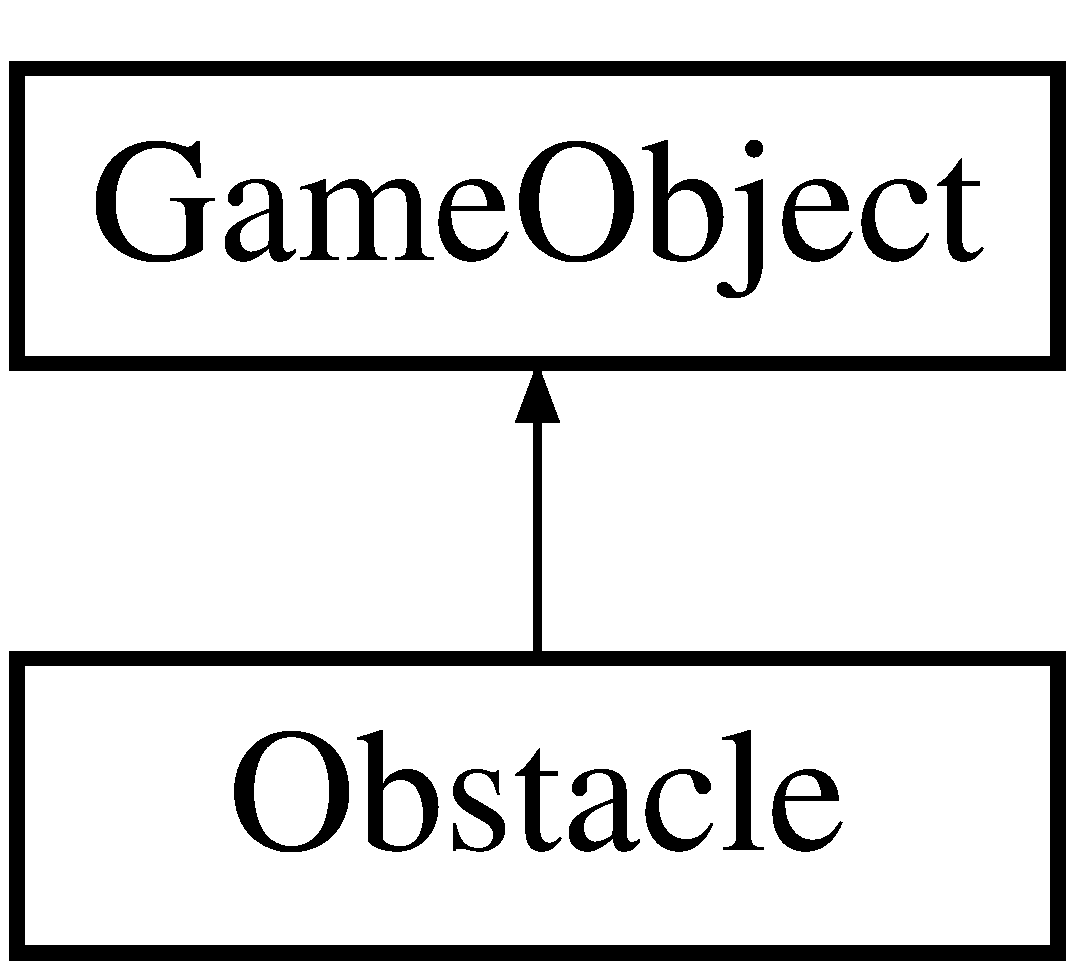
\includegraphics[height=2.000000cm]{classObstacle}
\end{center}
\end{figure}
\subsection*{Public Member Functions}
\begin{DoxyCompactItemize}
\item 
{\bfseries Obstacle} (\hyperlink{classVec4}{Vec4} const \+\_\+position, \hyperlink{classVec4}{Vec4} const \+\_\+rotation, float \+\_\+speed, bool \+\_\+active, int \+\_\+life, \hyperlink{classMesh}{Mesh} $\ast$\+\_\+mesh, float \+\_\+size)\hypertarget{classObstacle_a78a09081fd4ef17227497c4f1076f325}{}\label{classObstacle_a78a09081fd4ef17227497c4f1076f325}

\item 
void {\bfseries draw} () const \hypertarget{classObstacle_ac7e7e1ae0763fd7f60296999106a8615}{}\label{classObstacle_ac7e7e1ae0763fd7f60296999106a8615}

\end{DoxyCompactItemize}
\subsection*{Additional Inherited Members}


\subsection{Detailed Description}
inherits from \hyperlink{classGameObject}{Game\+Object} and is a static element in the scene 

The documentation for this class was generated from the following file\+:\begin{DoxyCompactItemize}
\item 
include/Obstacle.\+h\end{DoxyCompactItemize}

\hypertarget{classParticle}{}\section{Particle Class Reference}
\label{classParticle}\index{Particle@{Particle}}


is a single element that will move in the same direction at constant speed  




{\ttfamily \#include $<$Particle.\+h$>$}

\subsection*{Public Member Functions}
\begin{DoxyCompactItemize}
\item 
{\bfseries Particle} (\hyperlink{classMesh}{Mesh} $\ast$\+\_\+mesh)\hypertarget{classParticle_a5e3d06b6bef3954e12925c5afea900f6}{}\label{classParticle_a5e3d06b6bef3954e12925c5afea900f6}

\item 
void {\bfseries activate} (\hyperlink{classVec4}{Vec4} \+\_\+position, float \+\_\+rotation)\hypertarget{classParticle_a6cedea6d3a25699a50ff56d35dce6b6c}{}\label{classParticle_a6cedea6d3a25699a50ff56d35dce6b6c}

\item 
void {\bfseries update} ()\hypertarget{classParticle_a686aad22bf7a80a089e117bbc7f4b738}{}\label{classParticle_a686aad22bf7a80a089e117bbc7f4b738}

\item 
void {\bfseries deactivate} ()\hypertarget{classParticle_aaf1e8719527db4286c8154d43060b4e5}{}\label{classParticle_aaf1e8719527db4286c8154d43060b4e5}

\item 
void {\bfseries draw} () const \hypertarget{classParticle_a6a9c890bdf962bd4c0bec12c8765cc6c}{}\label{classParticle_a6a9c890bdf962bd4c0bec12c8765cc6c}

\end{DoxyCompactItemize}


\subsection{Detailed Description}
is a single element that will move in the same direction at constant speed 

The documentation for this class was generated from the following file\+:\begin{DoxyCompactItemize}
\item 
include/Particle.\+h\end{DoxyCompactItemize}

\hypertarget{classParticles}{}\section{Particles Class Reference}
\label{classParticles}\index{Particles@{Particles}}


handles the activation of multiple \hyperlink{classParticle}{Particle} objects  




{\ttfamily \#include $<$Particles.\+h$>$}

\subsection*{Public Member Functions}
\begin{DoxyCompactItemize}
\item 
{\bfseries Particles} (int \+\_\+particles, \hyperlink{classMesh}{Mesh} $\ast$m\+\_\+mesh)\hypertarget{classParticles_a72fe087ac7fb6d7af2903fb23deb2a6a}{}\label{classParticles_a72fe087ac7fb6d7af2903fb23deb2a6a}

\item 
void {\bfseries activate\+Particles} (\hyperlink{classVec4}{Vec4} \+\_\+position)\hypertarget{classParticles_a0e6a9f0d1d924e49c07d68206c88e2d4}{}\label{classParticles_a0e6a9f0d1d924e49c07d68206c88e2d4}

\item 
void {\bfseries update\+Particles} ()\hypertarget{classParticles_a0c796972d3b457121398ee9168363d1b}{}\label{classParticles_a0c796972d3b457121398ee9168363d1b}

\item 
void {\bfseries deactivate\+Particles} ()\hypertarget{classParticles_ad97778a640cfdf54fe67ec3abdaaad74}{}\label{classParticles_ad97778a640cfdf54fe67ec3abdaaad74}

\item 
void {\bfseries draw} () const \hypertarget{classParticles_aaf59f31d8ef8135350b87bf0f173c7a1}{}\label{classParticles_aaf59f31d8ef8135350b87bf0f173c7a1}

\end{DoxyCompactItemize}


\subsection{Detailed Description}
handles the activation of multiple \hyperlink{classParticle}{Particle} objects 

The documentation for this class was generated from the following file\+:\begin{DoxyCompactItemize}
\item 
include/Particles.\+h\end{DoxyCompactItemize}

\hypertarget{classPlayer}{}\section{Player Class Reference}
\label{classPlayer}\index{Player@{Player}}


is an Object controlled by a player  




{\ttfamily \#include $<$Player.\+h$>$}

Inheritance diagram for Player\+:\begin{figure}[H]
\begin{center}
\leavevmode
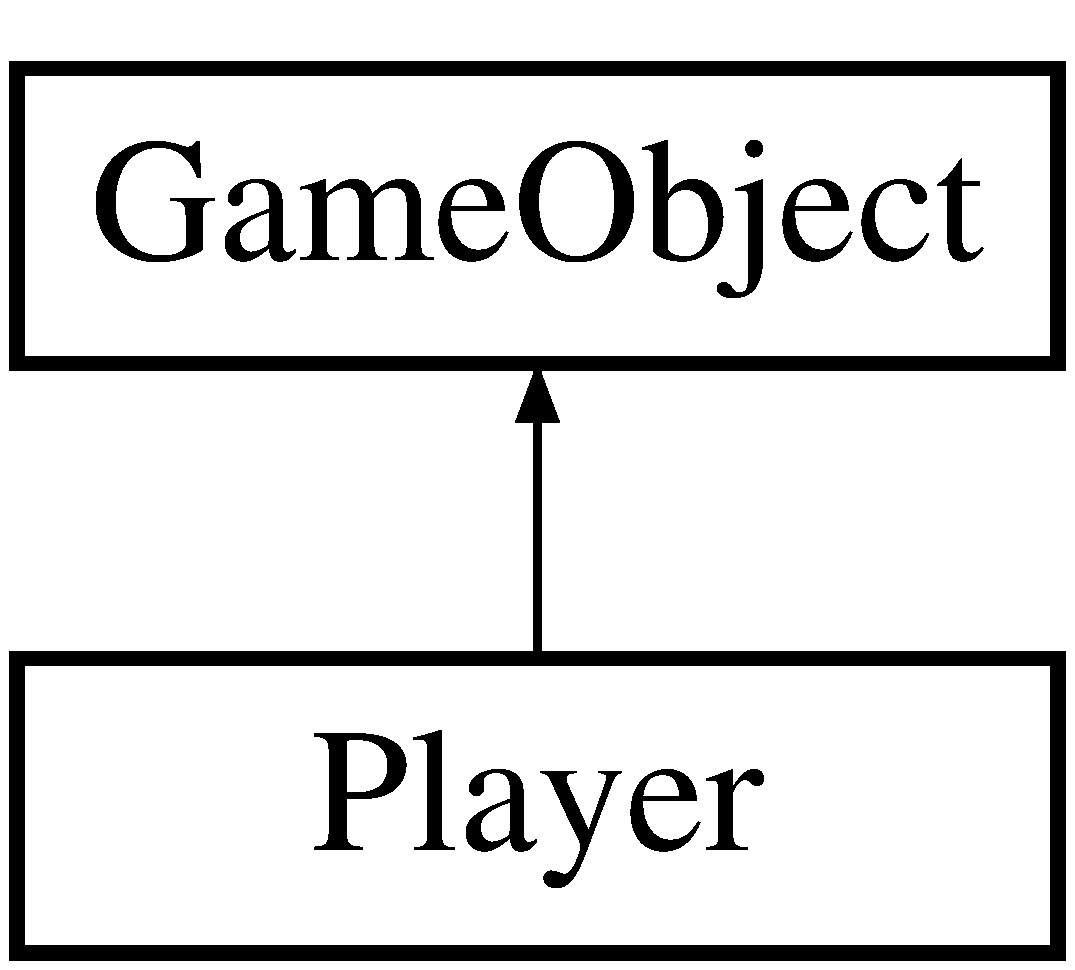
\includegraphics[height=2.000000cm]{classPlayer}
\end{center}
\end{figure}
\subsection*{Public Member Functions}
\begin{DoxyCompactItemize}
\item 
{\bfseries Player} (\hyperlink{classVec4}{Vec4} const \+\_\+position, \hyperlink{classVec4}{Vec4} const \+\_\+rotation, float \+\_\+speed, bool \+\_\+active, int \+\_\+life, \hyperlink{classMesh}{Mesh} $\ast$\+\_\+player\+Mesh)\hypertarget{classPlayer_aea2cc909f6edf32535322dc2e50e706d}{}\label{classPlayer_aea2cc909f6edf32535322dc2e50e706d}

\item 
void {\bfseries update\+Position} ()\hypertarget{classPlayer_a1cb7ff18fe3b07cc1dcd27519bde8329}{}\label{classPlayer_a1cb7ff18fe3b07cc1dcd27519bde8329}

\item 
void {\bfseries update\+Rotation} ()\hypertarget{classPlayer_a13b4bc20dd8e661bd091684a77e62762}{}\label{classPlayer_a13b4bc20dd8e661bd091684a77e62762}

\item 
void {\bfseries check\+Collision} (bool \+\_\+collided)\hypertarget{classPlayer_a2ce46af4329b7dd62de5314cfdf68d02}{}\label{classPlayer_a2ce46af4329b7dd62de5314cfdf68d02}

\item 
void {\bfseries draw} () const \hypertarget{classPlayer_aa1df31ab187c296318bb2ca09237e010}{}\label{classPlayer_aa1df31ab187c296318bb2ca09237e010}

\item 
bool {\bfseries can\+Shoot} () const \hypertarget{classPlayer_aea39f9314e03fe306eb46492ca441c8b}{}\label{classPlayer_aea39f9314e03fe306eb46492ca441c8b}

\item 
void {\bfseries can\+Shoot} (bool \+\_\+can\+Shoot)\hypertarget{classPlayer_ab01c82bacc9fe74dc30a278984cb30a8}{}\label{classPlayer_ab01c82bacc9fe74dc30a278984cb30a8}

\item 
void {\bfseries input} (S\+D\+L\+\_\+\+Event \&\+\_\+event)\hypertarget{classPlayer_aab63aa497bf58ad86b83f79568fd8763}{}\label{classPlayer_aab63aa497bf58ad86b83f79568fd8763}

\item 
\hyperlink{classVec4}{Vec4} {\bfseries get\+Next\+Position} () const \hypertarget{classPlayer_a86231b2071b967960041afb4578dc484}{}\label{classPlayer_a86231b2071b967960041afb4578dc484}

\item 
void {\bfseries will\+Collide} (bool \+\_\+will\+Collide)\hypertarget{classPlayer_a75fc22bdb8f6857f181eb85cc07efcc2}{}\label{classPlayer_a75fc22bdb8f6857f181eb85cc07efcc2}

\item 
std\+::array$<$ char, 5 $>$ {\bfseries pressed\+Keys} ()\hypertarget{classPlayer_ae0c6fe41ad92fc72437b38fe97422a58}{}\label{classPlayer_ae0c6fe41ad92fc72437b38fe97422a58}

\item 
void {\bfseries reset\+Life} ()\hypertarget{classPlayer_a2cd88e83a7839a42d68fb9f6965cc8a2}{}\label{classPlayer_a2cd88e83a7839a42d68fb9f6965cc8a2}

\item 
void {\bfseries updatehealth\+Bar} ()\hypertarget{classPlayer_a2b19a4da34d0b64209b617107c4d4ce7}{}\label{classPlayer_a2b19a4da34d0b64209b617107c4d4ce7}

\end{DoxyCompactItemize}
\subsection*{Additional Inherited Members}


\subsection{Detailed Description}
is an Object controlled by a player 

The documentation for this class was generated from the following file\+:\begin{DoxyCompactItemize}
\item 
include/Player.\+h\end{DoxyCompactItemize}

\hypertarget{classutilityFunctions}{}\section{utility\+Functions Class Reference}
\label{classutilityFunctions}\index{utility\+Functions@{utility\+Functions}}
\subsection*{Static Public Member Functions}
\begin{DoxyCompactItemize}
\item 
static std\+::vector$<$ std\+::string $>$ {\bfseries split} (const std\+::string \+\_\+string\+In, char \+\_\+split\+Char= \textquotesingle{} \textquotesingle{})\hypertarget{classutilityFunctions_a8d92ce117b8496eb26f975bb363228a0}{}\label{classutilityFunctions_a8d92ce117b8496eb26f975bb363228a0}

\item 
static std\+::vector$<$ std\+::string $>$ {\bfseries load\+From\+File} (const std\+::string \+\_\+file\+Name)\hypertarget{classutilityFunctions_a2f3dae0b035b1d4102c60a0328f574f2}{}\label{classutilityFunctions_a2f3dae0b035b1d4102c60a0328f574f2}

\item 
static std\+::vector$<$ std\+::array$<$ float, 3 $>$ $>$ {\bfseries get\+Vertices} (const std\+::vector$<$ std\+::string $>$ \+\_\+vector\+In)\hypertarget{classutilityFunctions_a87adf8e3dc58c0bf025aca153d988dda}{}\label{classutilityFunctions_a87adf8e3dc58c0bf025aca153d988dda}

\item 
static std\+::vector$<$ std\+::vector$<$ std\+::string $>$ $>$ {\bfseries get\+Faces} (const std\+::vector$<$ std\+::string $>$ \+\_\+vector\+In)\hypertarget{classutilityFunctions_add78b90c4c370f78955105b5ffe54ef7}{}\label{classutilityFunctions_add78b90c4c370f78955105b5ffe54ef7}

\item 
static std\+::vector$<$ std\+::array$<$ float, 3 $>$ $>$ {\bfseries get\+Normals} (const std\+::vector$<$ std\+::string $>$ \+\_\+vector\+In)\hypertarget{classutilityFunctions_a7f95611addb4e48faa286444cb22dec4}{}\label{classutilityFunctions_a7f95611addb4e48faa286444cb22dec4}

\item 
static void {\bfseries Draw\+Faces} (const std\+::vector$<$ std\+::array$<$ float, 3 $>$$>$ \+\_\+vertices, const std\+::vector$<$ std\+::array$<$ float, 3 $>$$>$ \+\_\+normals, std\+::vector$<$ std\+::vector$<$ std\+::string $>$$>$ \+\_\+faces, float size)\hypertarget{classutilityFunctions_acaa221ca126ccbf2aa9edf1fc4fc670c}{}\label{classutilityFunctions_acaa221ca126ccbf2aa9edf1fc4fc670c}

\item 
static void {\bfseries Draw\+Simple\+Level} ()\hypertarget{classutilityFunctions_aaf022cdf38d307c95c80fc3edde6021b}{}\label{classutilityFunctions_aaf022cdf38d307c95c80fc3edde6021b}

\item 
static std\+::vector$<$ char $>$ {\bfseries generate\+Obstacles} (const int \+\_\+x, const int \+\_\+z)\hypertarget{classutilityFunctions_a38938fe92753e93d58de256b1b7c77a5}{}\label{classutilityFunctions_a38938fe92753e93d58de256b1b7c77a5}

\item 
static void {\bfseries Draw\+Level} (const std\+::vector$<$ char $>$ \+\_\+map, const int \+\_\+x)\hypertarget{classutilityFunctions_a8b846904f8090abc4fa16e99a6e8ff3a}{}\label{classutilityFunctions_a8b846904f8090abc4fa16e99a6e8ff3a}

\end{DoxyCompactItemize}


The documentation for this class was generated from the following file\+:\begin{DoxyCompactItemize}
\item 
include/Utility\+Functions.\+h\end{DoxyCompactItemize}

\input{classutilityFunctions}
\hypertarget{classVec4}{}\section{Vec4 Class Reference}
\label{classVec4}\index{Vec4@{Vec4}}
\subsection*{Public Member Functions}
\begin{DoxyCompactItemize}
\item 
{\bfseries Vec4} (const \hyperlink{classVec4}{Vec4} \&\+\_\+rhs)=default\hypertarget{classVec4_a7fd0194b237680588058b50e8d80bee3}{}\label{classVec4_a7fd0194b237680588058b50e8d80bee3}

\item 
{\bfseries Vec4} (G\+Lfloat \+\_\+x=0.\+0f, G\+Lfloat \+\_\+y=0.\+0f, G\+Lfloat \+\_\+z=0.\+0f, G\+Lfloat \+\_\+w=1.\+0f)\hypertarget{classVec4_a88c48fa08f6b300577b374d3078186f8}{}\label{classVec4_a88c48fa08f6b300577b374d3078186f8}

\item 
void {\bfseries colour\+GL} () const \hypertarget{classVec4_ab6408ead37201958bbf4a9680b8d65a9}{}\label{classVec4_ab6408ead37201958bbf4a9680b8d65a9}

\item 
\hyperlink{classVec4}{Vec4} {\bfseries cross} (const \hyperlink{classVec4}{Vec4} \&\+\_\+rhs) const \hypertarget{classVec4_a5a2139b9f193e528e8f9bee0d0a14652}{}\label{classVec4_a5a2139b9f193e528e8f9bee0d0a14652}

\item 
float {\bfseries dot} (const \hyperlink{classVec4}{Vec4} \&\+\_\+rhs) const \hypertarget{classVec4_a91498b8d3af850201aababdeb523c58e}{}\label{classVec4_a91498b8d3af850201aababdeb523c58e}

\item 
float {\bfseries length} () const \hypertarget{classVec4_a08573e03357a6d14294da98c46cbab58}{}\label{classVec4_a08573e03357a6d14294da98c46cbab58}

\item 
float {\bfseries length\+Squared} () const \hypertarget{classVec4_ae2413a4eb232a55f15bafa13e49e75b7}{}\label{classVec4_ae2413a4eb232a55f15bafa13e49e75b7}

\item 
void {\bfseries normal\+GL} () const \hypertarget{classVec4_aefca6527cea99964c2075a02de8b341d}{}\label{classVec4_aefca6527cea99964c2075a02de8b341d}

\item 
void {\bfseries normalize} ()\hypertarget{classVec4_aecf9d5a3003c2a443098b4d80bc9dea6}{}\label{classVec4_aecf9d5a3003c2a443098b4d80bc9dea6}

\item 
\hyperlink{classVec4}{Vec4} {\bfseries operator$\ast$} (const \hyperlink{classMat4}{Mat4} \&\+\_\+r) const \hypertarget{classVec4_a878f420e799f587d908da586afd654c5}{}\label{classVec4_a878f420e799f587d908da586afd654c5}

\item 
\hyperlink{classVec4}{Vec4} {\bfseries operator$\ast$} (G\+Lfloat \+\_\+rhs) const \hypertarget{classVec4_ab3802d9f4dee81313994294ee6718c82}{}\label{classVec4_ab3802d9f4dee81313994294ee6718c82}

\item 
void {\bfseries operator$\ast$=} (G\+Lfloat \+\_\+rhs)\hypertarget{classVec4_ac0efcc6b09bc660cd42072a15b83b8bd}{}\label{classVec4_ac0efcc6b09bc660cd42072a15b83b8bd}

\item 
\hyperlink{classVec4}{Vec4} {\bfseries operator+} (const \hyperlink{classVec4}{Vec4} \&\+\_\+rhs) const \hypertarget{classVec4_a58014ec694674a8c27587a03037f0f09}{}\label{classVec4_a58014ec694674a8c27587a03037f0f09}

\item 
void {\bfseries operator+=} (const \hyperlink{classVec4}{Vec4} \&\+\_\+rhs)\hypertarget{classVec4_a9d7dbf4c6dc031cbed8a0d5938021821}{}\label{classVec4_a9d7dbf4c6dc031cbed8a0d5938021821}

\item 
\hyperlink{classVec4}{Vec4} {\bfseries operator-\/} (const \hyperlink{classVec4}{Vec4} \&\+\_\+rhs) const \hypertarget{classVec4_ae2579c5b5ce533033325ebd78bf3d544}{}\label{classVec4_ae2579c5b5ce533033325ebd78bf3d544}

\item 
bool {\bfseries operator==} (const \hyperlink{classVec4}{Vec4} \&\+\_\+rhs) const \hypertarget{classVec4_a179aabcc9171e5daeb9d95503ecf86af}{}\label{classVec4_a179aabcc9171e5daeb9d95503ecf86af}

\item 
G\+Lfloat \& {\bfseries operator\mbox{[}$\,$\mbox{]}} (int \+\_\+i)\hypertarget{classVec4_a0fde5c8772ebb5e0f833bd56f16d04f9}{}\label{classVec4_a0fde5c8772ebb5e0f833bd56f16d04f9}

\item 
void {\bfseries set} (G\+Lfloat \+\_\+x, G\+Lfloat \+\_\+y, G\+Lfloat \+\_\+z, G\+Lfloat \+\_\+w=1.\+0f)\hypertarget{classVec4_a63f1350537ea2b3fdf564627a4b23757}{}\label{classVec4_a63f1350537ea2b3fdf564627a4b23757}

\item 
void {\bfseries vertex\+GL} () const \hypertarget{classVec4_ae637ea15f081d10860629ec70f95929a}{}\label{classVec4_ae637ea15f081d10860629ec70f95929a}

\end{DoxyCompactItemize}
\subsection*{Public Attributes}
\begin{DoxyCompactItemize}
\item 
\begin{tabbing}
xx\=xx\=xx\=xx\=xx\=xx\=xx\=xx\=xx\=\kill
union \{\\
\>GLfloat {\bfseries m\_openGL} \mbox{[}4\mbox{]}\\
\>struct \{\\
\>\>GLfloat {\bfseries m\_x}\\
\>\>GLfloat {\bfseries m\_y}\\
\>\>GLfloat {\bfseries m\_z}\\
\>\>GLfloat {\bfseries m\_w}\\
\>\} \hypertarget{unionVec4_1_1_0D4_afd2b5891329ef3fc9b8a749eab8b0008}{}\label{unionVec4_1_1_0D4_afd2b5891329ef3fc9b8a749eab8b0008}
\\
\}; \hypertarget{classVec4_a8f0e755891bc3e425a0dcc2d95271128}{}\label{classVec4_a8f0e755891bc3e425a0dcc2d95271128}
\\

\end{tabbing}\end{DoxyCompactItemize}


The documentation for this class was generated from the following file\+:\begin{DoxyCompactItemize}
\item 
G\+L\+Functions\+Lib/include/Vec4.\+h\end{DoxyCompactItemize}

\hypertarget{classWindow}{}\section{Window Class Reference}
\label{classWindow}\index{Window@{Window}}


initializes Open\+GL and S\+DL and creates a window  




{\ttfamily \#include $<$Window.\+h$>$}

\subsection*{Public Member Functions}
\begin{DoxyCompactItemize}
\item 
{\bfseries Window} (const int \+\_\+width, const int \+\_\+height)\hypertarget{classWindow_a7a2b8f008b7abfbb094e919e11340b54}{}\label{classWindow_a7a2b8f008b7abfbb094e919e11340b54}

\item 
int {\bfseries get\+Width} () const \hypertarget{classWindow_ad6c886b8b3b4034c2ad034bba30e4244}{}\label{classWindow_ad6c886b8b3b4034c2ad034bba30e4244}

\item 
int {\bfseries get\+Height} () const \hypertarget{classWindow_ab212a935b7e5bb15fe5bc1784725c1b1}{}\label{classWindow_ab212a935b7e5bb15fe5bc1784725c1b1}

\item 
void {\bfseries set\+Window\+Size} (const int \&\+\_\+width, const int \&\+\_\+height)\hypertarget{classWindow_acab1d14669c60a860b7b309b019f3d66}{}\label{classWindow_acab1d14669c60a860b7b309b019f3d66}

\item 
S\+D\+L\+\_\+\+Window $\ast$ {\bfseries get\+Window} () const \hypertarget{classWindow_adf523e859cb409c999bc8f349b879afb}{}\label{classWindow_adf523e859cb409c999bc8f349b879afb}

\item 
S\+D\+L\+\_\+\+Renderer $\ast$ {\bfseries get\+Renderer} () const \hypertarget{classWindow_af2bcfa04cbce391c7a31fe30aa8511b7}{}\label{classWindow_af2bcfa04cbce391c7a31fe30aa8511b7}

\end{DoxyCompactItemize}


\subsection{Detailed Description}
initializes Open\+GL and S\+DL and creates a window 

The documentation for this class was generated from the following file\+:\begin{DoxyCompactItemize}
\item 
include/Window.\+h\end{DoxyCompactItemize}

%--- End generated contents ---

% Index
\backmatter
\newpage
\phantomsection
\clearemptydoublepage
\addcontentsline{toc}{chapter}{Index}
\printindex

\end{document}
